\documentclass[11pt]{article}
\usepackage[margin=1in]{geometry}
\usepackage{amsmath,amssymb,amsthm,mathtools}
\usepackage{booktabs}
\usepackage{tikz}
\usetikzlibrary{positioning}

\newtheorem{theorem}{Theorem}
\newtheorem{proposition}[theorem]{Proposition}
\newtheorem{lemma}[theorem]{Lemma}
\newtheorem{corollary}[theorem]{Corollary}
\newcommand{\Bd}{\mathrm{Bd}}
\newcommand{\dB}{\mathrm{dB}}
\newcommand{\rhoU}[3]{\rho_{#1}(#2,#3)}

\title{A Sharp Strong-Selection Obstruction to\\
Universal Simultaneous Amplification}
\author{}
\date{August 1, 2026}

\begin{document}
\maketitle

\begin{abstract}
We ask whether a finite connected undirected weighted graph can strictly
increase uniformly initialized single-mutant fixation probability, relative
to the same-order complete graph, under both birth--death and death--birth
updating for every mutant fitness $r>1$.  We prove a stronger negative result:
no such graph is an all-fitness amplifier even for death--birth updating alone.
If the positive-weight support is incomplete, its death--birth fixation
probability has a strictly smaller strong-selection limit.  If the support is
complete, its first $1/r$ correction is no better than the complete graph's,
and the excess loss has an explicit sum-of-squares certificate.  Equality
forces all edge weights to be equal, in which case the process is exactly the
complete-graph baseline.  The obstruction applies to every finite graph and
therefore rules out every fitness-independent graph family.
\end{abstract}

\section{Relation to prior bounds}

Tkadlec et al. proved that every noncomplete population structure---even with
directed or weighted edges---is eventually dB-suppressing as fitness grows
\cite{Tkadlec2020}.  Their theorem explicitly
leaves one residual possibility: a nonuniform weighted version of the complete
graph.  They list universal dB amplification as an open direction and observe
that any example would have to lie in that class.  The complete-support branch
of our theorem closes this residual case for finite undirected symmetric
loopless weights.  Its $1/r$ coefficient also provides an equality
characterization not supplied by the earlier average-degree bound.

Transient dB amplification is known and can be diagnosed at weak selection
using coalescing random walks \cite{Allen2020}.  More recently, weighted modular
graphs have been proved to amplify both Bd and dB selection on the fixed fitness
interval $(1,1.2)$ \cite{Svoboda2024}.  Those positive results are consistent
with the obstruction here: our conclusion concerns a single graph required to
amplify for every $r>1$, and failure occurs in its strong-selection tail.

\section{Model and result}

Let $G=(V,w)$ be a connected loopless undirected weighted graph, with
$|V|=n\ge2$, $w_{ij}=w_{ji}\ge0$, and every weighted degree positive.  Mutants
have fitness $r>1$ and residents fitness one.  Under death--birth updating a
uniformly chosen vertex dies, after which a neighbor is chosen for reproduction
with probability proportional to fitness times edge weight.  Write
$\rho_{\dB}(G,r)$ for fixation probability averaged uniformly over all
single-mutant initial vertices.  Let
\[
 s_i=|\{j:w_{ij}>0\}|
\]
be the degree of $i$ in the positive-weight support.

\begin{theorem}[sharp strong-selection obstruction]\label{thm:main}
For every finite connected undirected weighted graph $G$ on $n\ge2$ vertices:
\begin{enumerate}
\item
\[
 \lim_{r\to\infty}\rho_{\dB}(G,r)
 =\frac1n\sum_i\frac{s_i}{s_i+1}.
\]
If the support is incomplete, then
\[
 \lim_{r\to\infty}
 \bigl(\rho_{\dB}(K_n,r)-\rho_{\dB}(G,r)\bigr)
 =\sum_i\frac{n-1-s_i}{n^2(s_i+1)}>0.
\]
\item Suppose the support is complete and $n\ge3$.  Put
\[
 \mathcal E(G)=
 \sum_i\sum_{\substack{j<k\\j,k\ne i}}
 \frac{(w_{ij}-w_{ik})^2}{w_{ij}w_{ik}}.
\]
Then
\[
 \rho_{\dB}(K_n,r)-\rho_{\dB}(G,r)
 =\frac{\mathcal E(G)}{n^2(n-2)r}+O(r^{-2}).
\]
Moreover, $\mathcal E(G)=0$ if and only if all off-diagonal weights are one
common positive constant.
\item For $n=2$, every admissible graph is a global rescaling of $K_2$, and
$\rho_{\dB}(G,r)=1/2$ for all $r$.
\end{enumerate}
Consequently every graph not equivalent to $K_n$ is strictly dB-suppressed
for all sufficiently large finite $r$, while a scaled $K_n$ ties the baseline
for every $r$.  No graph, and hence no fitness-independent graph family, is a
strict dB amplifier for every $r>1$; in particular universal simultaneous
Bd/dB amplification is impossible.
\end{theorem}

The two branches of the certificate are shown schematically in
Figure~\ref{fig:dichotomy}.

\begin{figure}[ht]
\centering
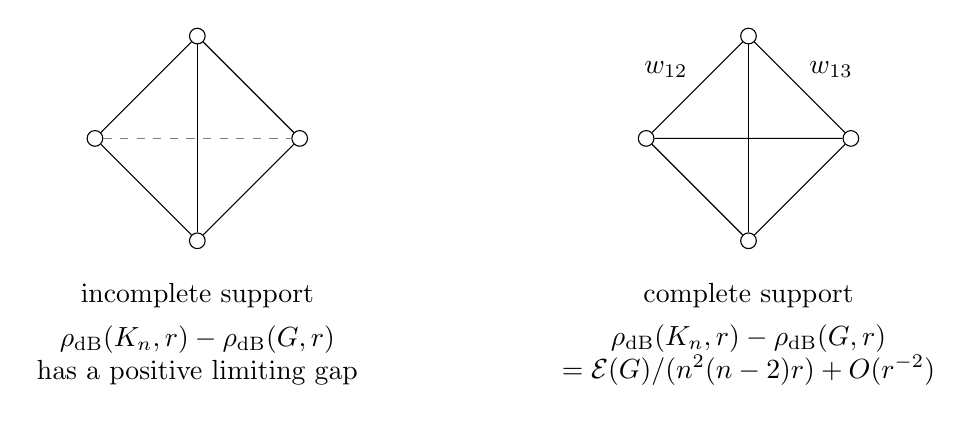
\begin{tikzpicture}[vertex/.style={circle,draw,fill=white,inner sep=2pt},
                    scale=1.0]
  \begin{scope}[xshift=-3.5cm]
    \node[vertex] (a) at (0,1.3) {};
    \node[vertex] (b) at (-1.3,0) {};
    \node[vertex] (c) at (1.3,0) {};
    \node[vertex] (d) at (0,-1.3) {};
    \draw (a)--(b)--(d)--(c)--(a);
    \draw (a)--(d);
    \draw[dashed,gray] (b)--(c);
    \node at (0,-2.0) {incomplete support};
    \node[align=center] at (0,-2.75)
      {$\displaystyle \rho_{\dB}(K_n,r)-\rho_{\dB}(G,r)$\\
       has a positive limiting gap};
  \end{scope}
  \begin{scope}[xshift=3.5cm]
    \node[vertex] (a) at (0,1.3) {};
    \node[vertex] (b) at (-1.3,0) {};
    \node[vertex] (c) at (1.3,0) {};
    \node[vertex] (d) at (0,-1.3) {};
    \draw (a)--node[above left] {$w_{12}$}(b);
    \draw (a)--node[above right] {$w_{13}$}(c);
    \draw (a)--(d);
    \draw (b)--(c) (b)--(d) (c)--(d);
    \node at (0,-2.0) {complete support};
    \node[align=center] at (0,-2.75)
      {$\displaystyle \rho_{\dB}(K_n,r)-\rho_{\dB}(G,r)$\\
       $\displaystyle =\mathcal E(G)/(n^2(n-2)r)+O(r^{-2})$};
  \end{scope}
\end{tikzpicture}
\caption{The exhaustive support dichotomy.  The dashed segment on the left is
a missing edge of the positive-weight support, not an edge weight to be
optimized.}
\label{fig:dichotomy}
\end{figure}

\section{Complete-graph baselines}

We derive both baselines directly.  Let $\phi_k$ denote fixation probability
on $K_n$ from $k$ mutants, and let $p_k^+$ and $p_k^-$ be the probabilities of
increasing and decreasing $k$.  The first-step equations give
\[
 p_k^+(\phi_{k+1}-\phi_k)=p_k^-(\phi_k-\phi_{k-1}).
\]
If $\gamma_k=p_k^-/p_k^+$, summing successive increments subject to
$\phi_0=0$ and $\phi_n=1$ gives
\[
 \phi_1=\left(1+\sum_{j=1}^{n-1}\prod_{k=1}^j\gamma_k\right)^{-1}.
\]

For Bd updating, $\gamma_k=1/r$, hence
\begin{equation}\label{eq:Bd-baseline}
 \rho_{\Bd}(K_n,r)=\frac{1-r^{-1}}{1-r^{-n}}.
\end{equation}
For dB updating, direct counting gives
\[
 p_k^+=\frac{n-k}{n}\frac{rk}{rk+n-k-1},\qquad
 p_k^-=\frac{k}{n}\frac{n-k}{r(k-1)+n-k}.
\]
Writing $A_k=n-1+(r-1)k$, one has
\[
 \gamma_k=\frac{A_k}{rA_{k-1}},\qquad
 \prod_{k=1}^j\gamma_k=\frac{A_j}{(n-1)r^j}.
\]
The finite sum telescopes to the exact formula
\begin{equation}\label{eq:dB-baseline}
 \rho_{\dB}(K_n,r)
 =\frac{n-1}{n}\frac{1-r^{-1}}{1-r^{-(n-1)}}.
\end{equation}
For $n\ge3$ this has the strong-selection expansion
\begin{equation}\label{eq:dB-baseline-expansion}
 \rho_{\dB}(K_n,r)
 =\frac{n-1}{n}-\frac{n-1}{nr}+O(r^{-2}).
\end{equation}

We will use the following elementary finite-chain perturbation fact to make
the $r\to\infty$ passage precise.

\begin{lemma}[finite-state perturbation]\label{lem:perturbation}
Let $P(\varepsilon)$ be a finite family of transition matrices continuous at
$\varepsilon=0$.  Suppose that, from a specified initial state, all states
reachable before absorption at $\varepsilon=0$ lie in a set $\mathcal R$, the
transient restriction $Q_{\mathcal R}(0)$ has spectral radius less than one,
and the one-step probability of leaving $\mathcal R$ is $O(\varepsilon)$.
Then the absorption probabilities converge to those of $P(0)$.  If
$\mathcal R$ is the full transient state space and the entries are analytic,
then the absorption probabilities are analytic near zero.
\end{lemma}

\begin{proof}
The inverse $(I-Q_{\mathcal R}(\varepsilon))^{-1}$ exists and remains bounded
for all sufficiently small $\varepsilon$.  Multiplying it by the vector of
one-step leakage probabilities shows that the probability of leaving
$\mathcal R$ before absorption is $O(\varepsilon)$.  The absorption equations
within $\mathcal R$ therefore converge to the nonsingular limiting system;
behavior after leakage can change a hitting probability by at most the
leakage probability.  In the full-space analytic case,
$(I-Q(\varepsilon))^{-1}$ is analytic by the adjugate formula.
\end{proof}

\section{Incomplete positive-weight support}

Fix an initial mutant vertex $i$.  At $r=\infty$, death of $i$ causes
extinction.  Death of any one of its $s_i$ support-neighbors is followed by
mutant reproduction with probability one and creates an adjacent mutant pair.
Deaths at nonneighbors are self-loops.  Conditioning on the first state change
therefore gives probability $s_i/(s_i+1)$ of reaching a pair before
extinction.

Once an adjacent pair has formed, the mutant set remains support-connected.
Every mutant has a mutant neighbor and hence cannot be replaced by a resident
in the limiting chain.  Whenever a boundary resident dies it becomes mutant.
Connectedness of the support implies monotone growth to fixation almost
surely.  Thus
\[
 \lim_{r\to\infty}\rho_{\dB}(G,r)
 =\frac1n\sum_i\frac{s_i}{s_i+1}.
\]
Subtracting this from $(n-1)/n$ gives the exact termwise certificate below.
\par\medskip
\begin{equation}\label{eq:support-gap}
 \frac{n-1}{n}-\frac1n\sum_i\frac{s_i}{s_i+1}
 =\sum_i\frac{n-1-s_i}{n^2(s_i+1)}.
\end{equation}
\smallskip
Every denominator is positive.  If an edge is missing, at least one numerator
is positive, proving the first branch of Theorem~\ref{thm:main}.

For completeness, the limiting argument is stable: from a singleton, every
limiting state reached before absorption is a connected mutant set.  The
finite limiting transient chain absorbs almost surely, so its fundamental
matrix is nonsingular.  For finite $r=1/\varepsilon$, a transition that leaks
from this set requires a resident to replace a mutant having a mutant
neighbor, and has probability $O(\varepsilon)$ in each fixed state.  Lemma
\ref{lem:perturbation} therefore proves convergence of the finite-$r$ hitting
probabilities, including the effect of all paths after such leakage.

\section{Complete support and the sum-of-squares correction}

Assume $n\ge3$ and $w_{ij}>0$ for all $i\ne j$.  Put
\[
 d_i=\sum_{j\ne i}w_{ij},\qquad \varepsilon=r^{-1},\qquad
 a_{ij}=\frac{d_i-w_{ij}}{w_{ij}}.
\]
Let $q_S(\varepsilon)$ be extinction probability from mutant set $S$.  At
$\varepsilon=0$, every set with at least two mutants fixates, while
$q_{\{i\}}(0)=1/n$.  The limiting transient chain absorbs almost surely, so
Lemma~\ref{lem:perturbation} shows that the hitting probabilities are analytic
near $\varepsilon=0$.

The first-order equations for $|S|\ge3$ have no forcing: a rare loss still
leaves at least two mutants, whose zeroth-order extinction probability is
zero.  Backward induction from the full state gives
\[
 q_S(\varepsilon)=O(\varepsilon^2),\qquad |S|\ge3.
\]

For $S=\{i,j\}$, loss of mutant $i$ occurs with probability
\[
 \frac1n\frac{\varepsilon(d_i-w_{ij})}
 {w_{ij}+\varepsilon(d_i-w_{ij})}
 =\frac{\varepsilon a_{ij}}n+O(\varepsilon^2),
\]
and similarly for $j$.  The leading self-loop probability is $2/n$ and the
leading total gain probability is $(n-2)/n$.  Since a resulting singleton has
extinction probability $1/n+O(\varepsilon)$, the exact first-step equation
gives, on putting
\[
 b_{ij}=\frac{a_{ij}+a_{ji}}{n(n-2)},
\]
\begin{equation}\label{eq:pair}
 q_{\{i,j\}}(\varepsilon)=b_{ij}\varepsilon+O(\varepsilon^2).
\end{equation}

From singleton $\{i\}$, death of resident $j$ creates $\{i,j\}$ with
probability
\[
 t_{ij}=\frac1n\frac{w_{ij}}
 {w_{ij}+\varepsilon(d_j-w_{ij})}
 =\frac1n(1-a_{ji}\varepsilon)+O(\varepsilon^2).
\]
Death of $i$ causes extinction with probability exactly $1/n$; every other
outcome is a self-loop.  Hence
\[
 \left(\frac1n+\sum_{j\ne i}t_{ij}\right)q_{\{i\}}
 =\frac1n+\sum_{j\ne i}t_{ij}q_{\{i,j\}}.
\]
Substitution of \eqref{eq:pair}, followed by uniform averaging, yields
\[
 T(G)=\sum_i\sum_{j\ne i}a_{ij},\qquad
 A(G)=\frac{T(G)}{n^2(n-2)},
\]
\begin{equation}\label{eq:full-expansion}
 \rho_{\dB}(G,r)
 =\frac{n-1}{n}-\frac{A(G)}r+O(r^{-2}).
\end{equation}

For the unit complete graph, $a_{ij}=n-2$ and
$T(K_n)=n(n-1)(n-2)$.  The difference admits the exact identity
\begin{align}
 T(G)-n(n-1)(n-2)
 &=\sum_i\left[
 d_i\sum_{j\ne i}\frac1{w_{ij}}-(n-1)^2\right] \notag\\
 &=\sum_i\sum_{\substack{j<k\\j,k\ne i}}
 \frac{(w_{ij}-w_{ik})^2}{w_{ij}w_{ik}}
 =\mathcal E(G).                                      \label{eq:sos}
\end{align}
All denominators in \eqref{eq:sos} are positive.  Equality requires every
star of incident weights to be constant; symmetry and complete support then
force one global edge weight.  Equations
\eqref{eq:dB-baseline-expansion}, \eqref{eq:full-expansion}, and
\eqref{eq:sos} prove the second branch of Theorem~\ref{thm:main}.

\section{Exact verification}

The accompanying verifier is separate from the discovery implementation.  It
constructs all subset-state transitions directly over $\mathbb Q(r)$, checks
row normalization and termwise positivity after the substitution $r=1+x$,
verifies strong lumpability of $K_n$ by mutant count, solves the exact
absorbing equations, and extracts the limiting coefficients.

As one nontrivial replay, take a weighted triangle with edge weights
$(w_{12},w_{13},w_{23})=(2,3,5)$.  Exact elimination gives
\[
 \rho_{\dB}(G,r)-\rho_{\dB}(K_3,r)
 =-\frac{r(r-1)P(r)}{9(r+1)Q(r)},
\]
where
\[
 \begin{aligned}
 P(r)&=900r^4+5491r^3+9290r^2+5491r+900,\\
 Q(r)&=675r^6+6600r^5+21791r^4+31768r^3\\
     &\hspace{2.7cm}{}+21791r^2+6600r+675.
 \end{aligned}
\]
Every displayed denominator factor is positive and the numerator is strictly
negative for $r>1$.  The verifier also recovers the strong coefficient
$22/27>2/3$, and recovers $343/320>3/4$ for the complete four-vertex weighting
with lexicographic edge weights $(1,2,3,4,5,6)$.  For incomplete support it
recovers limits $7/12$ for the four-vertex path and $9/16$ for the four-vertex
star, against the baseline $3/4$.

These calculations are checks, not evidence used to extend a finite search:
the universal quantifier is discharged by the exact certificates
\eqref{eq:support-gap} and \eqref{eq:sos}.

\section{Finite versus asymptotic statements}

The expansions in Theorem~\ref{thm:main} are taken separately for each fixed
finite graph.  They imply that for every nonbaseline $G$ there exists a finite
threshold $R_G$ such that
\[
 \rho_{\dB}(G,r)<\rho_{\dB}(K_n,r)\qquad(r>R_G).
\]
No claim of a graph-independent threshold is needed.  The all-$r$ amplifier
property quantifies over every finite $r>1$ for each graph, so the existence of
one such suppressing tail already rules it out.  The equality case is exact,
not asymptotic: global rescaling cancels from every neighbor-choice
probability, so a uniformly weighted complete graph has precisely the
baseline chain for all finite $r$.

\begin{thebibliography}{9}

\bibitem{Tkadlec2020}
J. Tkadlec, A. Pavlogiannis, K. Chatterjee, and M. A. Nowak,
``Limits on amplifiers of natural selection under death--Birth updating,''
\emph{PLoS Computational Biology} 16 (2020), e1007494.
\texttt{doi:10.1371/journal.pcbi.1007494}.

\bibitem{Allen2020}
B. Allen, C. Sample, R. Jencks, J. Withers, P. Steinhagen, L. Brizuela,
J. Kolodny, D. Parke, G. Lippner, and Y. A. Dementieva,
``Transient amplifiers of selection and reducers of fixation for death--Birth
updating on graphs,'' \emph{PLoS Computational Biology} 16 (2020), e1007529.
\texttt{doi:10.1371/journal.pcbi.1007529}.

\bibitem{Svoboda2024}
J. Svoboda, S. S. Joshi, J. Tkadlec, and K. Chatterjee,
``Amplifiers of selection for the Moran process with both Birth--death and
death--Birth updating,'' \emph{PLoS Computational Biology} 20 (2024), e1012008.
\texttt{doi:10.1371/journal.pcbi.1012008}.

\end{thebibliography}

\end{document}
